\section{To‘la ichki qaytish}


\begin{enumerate}

\item Yorug‘lik nuri sindirish ko‘rsatkichi $n_1$ bo‘lgan muhitdan sindirish ko‘rsatkichi $n_2$ bo‘lgan muhitga o‘tganda, to‘la qaytishning chegaraviy burchagi qaysi ifoda yordamida aniqlanadi? $(n_1>n_2)$
\begin{enumerate}[label=\Alph*)]
\item $\sin\alpha_0=\dfrac{n_1}{n_2}$
\item $\sin\alpha_0=\dfrac{1}{n_1}$
\item $\sin\alpha_0=\dfrac{n_2}{n_1}$
\item $\sin\alpha_0=\dfrac{1}{n_2}$
\item TJY.
\end{enumerate}

\item Yorug‘lik nuri absolyut sindirish ko‘rsatkichi $2$ bo‘lgan muhitdan vakuumga o‘tmoqda. To‘la ichki qaytish sodir bo‘ladigan tushish burchagining eng kichik qiymatini toping.
\begin{enumerate}[label=\Alph*)]
\item $30^\circ$
\item $45^\circ$
\item $60^\circ$
\item $75^\circ$
\item $90^\circ$
\end{enumerate}

\item Yorug‘lik nuri absolyut sindirish ko‘rsatkichi $2\sqrt{2}$ bo‘lgan muhitdan absolyut sindirish ko‘rsatkichi $\sqrt{2}$ bo‘lgan muhitga o‘tdi. To‘la ichki qaytishning chegaraviy burchagini toping.
\begin{enumerate}[label=\Alph*)]
\item $30^\circ$
\item $45^\circ$
\item $60^\circ$
\item $75^\circ$
\item $90^\circ$
\end{enumerate}

\item Yorug‘lik nuri absolyut sindirish ko‘rsatkichi $n_1$ bo‘lgan muhitdan absolyut sindirish ko‘rsatkichi $\sqrt{2}$ bo‘lgan muhitga o‘tdi. To‘la ichki qaytish sodir bo‘ladigan tushish burchagining eng kichik qiymati $45^\circ$ ga teng bo‘lsa, $n_1$ ning qiymatini toping.
\begin{enumerate}[label=\Alph*)]
\item $3$
\item $2\sqrt{2}$
\item $1,5$
\item $\sqrt{3}$
\item $2$
\end{enumerate}

\item Yorug‘lik nuri absolyut sindirish ko‘rsatkichi $2\sqrt{3}$ bo‘lgan muhitdan absolyut sindirish ko‘rsatkichi $n_2$ bo‘lgan muhitga o‘tdi. To‘la ichki qaytishning chegaraviy burchagi $60^\circ$ ga teng bo‘lsa, $n_2$ ni toping.
\begin{enumerate}[label=\Alph*)]
\item $3$
\item $2\sqrt{2}$
\item $1,5$
\item $\sqrt{3}$
\item $2$
\end{enumerate}

\item Yorug‘lik nuri absolyut sindirish ko‘rsatkichi $2$ bo‘lgan muhitdan absolyut sindirish ko‘rsatkichi $3$ bo‘lgan muhitga o‘tdi. To‘la ichki qaytishning chegaraviy burchagini toping.
\begin{enumerate}[label=\Alph*)]
\item $30^\circ$
\item $45^\circ$
\item $60^\circ$
\item $75^\circ$
\item to‘la ichki qaytish sodir bo‘lmaydi.
\end{enumerate}

\item Yorug‘lik nuri absolyut sindirish ko‘rsatkichi $\sqrt{2}$ bo‘lgan muhitdan vakuumga o‘tmoqda. To‘la ichki qaytishning chegaraviy burchagini toping.
\begin{enumerate}[label=\Alph*)]
\item $30^\circ$
\item $45^\circ$
\item $60^\circ$
\item $75^\circ$
\item to‘la ichki qaytish sodir bo‘lmaydi.
\end{enumerate}

\item Yorug‘lik nuri absolyut sindirish ko‘rsatkichi $2$ bo‘lgan muhitdan absolyut sindirish ko‘rsatkichi $\sqrt{3}$ bo‘lgan muhitga o‘tdi. To‘la ichki qaytish sodir bo‘ladigan tushish burchagining eng kichik qiymatini toping.
\begin{enumerate}[label=\Alph*)]
\item $30^\circ$
\item $45^\circ$
\item $60^\circ$
\item $75^\circ$
\item to‘la ichki qaytish sodir bo‘lmaydi.
\end{enumerate}

\item Yorug‘lik nuri vakuumdan absolyut sindirish ko‘rsatkichi $2$ bo‘lgan muhitga o‘tdi. To‘la ichki qaytishning chegaraviy burchagini toping.
\begin{enumerate}[label=\Alph*)]
\item $30^\circ$
\item $45^\circ$
\item $60^\circ$
\item $75^\circ$
\item to‘la ichki qaytish sodir bo‘lmaydi.
\end{enumerate}

\item Yorug‘lik sindirish ko‘rsatkichi $n_1$ bo‘lgan muhitdan $n_2$ bo‘lgan muhitga o‘tmoqda. Quyidagilardan qaysi shart bajarilganda to‘la ichki qaytish yuzaga keladi?
\begin{enumerate}[label=\Alph*)]
\item $n_1>n_2$.
\item $n_1<n_2$.
\item $n_1=n_2$.
\item sindirish ko‘rsatkichlarining to‘la ichki qaytishga ta’siri yo‘q.
\item TJY.
\end{enumerate}

\item Nur sindirish ko‘rsatkichi $n$ bo‘lgan shisha plastinka ichida tarqalib, shisha–havo chegarasiga $\alpha$ burchak ostida tushyapti (rasm). Agar bu burchak to‘la ichki qaytishning chegaraviy burchagi teng bo‘lsa, singan va qaytgan nurlar orasidagi burchak teng bo‘ladi?

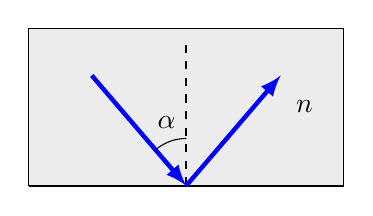
\begin{tikzpicture}[>=latex, scale=1]
    % Muhitni ifodalovchi to'rtburchak va fon
    \fill[gray!15] (-2,0) rectangle (2,2);
    \draw[thick] (-2,0) -- (2,0); % Pastki sirt
    \draw (-2,2) -- (2,2) -- (2,0); % Chegaralar
    \draw (-2,2) -- (-2,0);

    % Normal (punktir chiziq)
    \draw[dashed, thick] (0,0) -- (0,1.8);
    
    % Nurlar (tushayotgan va qaytayotgan)
    \draw[ultra thick, blue, ->] (-1.2, 1.4) -- (0,0);
    \draw[ultra thick, blue, ->] (0,0) -- (1.2, 1.4);
    
    % Alfa burchagi
    \draw (0,0.6) arc (90:131:0.6);
    \node at (-0.25, 0.8) {$\alpha$};
    
    % Muhit belgisi n
    \node at (1.5, 1) {$n$};
\end{tikzpicture}

\begin{enumerate}[label=\Alph*)]
\item $90^\circ+\alpha$
\item $\alpha$
\item $2\alpha$
\item $90^\circ-\alpha$
\item $0$
\end{enumerate}

\item Tushish burchagi $\alpha$ qanday bo‘lganda yorug‘likning to‘la ichki qaytish hodisasi ro‘y beradi?

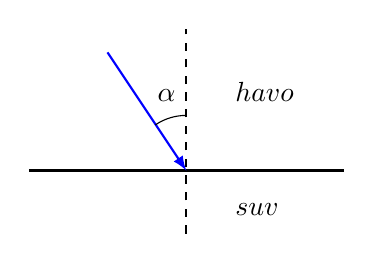
\begin{tikzpicture}[>=latex, scale=1]
    % Muhitlar chegarasi (horizontal chiziq)
    \draw[thick] (-2,0) -- (2,0);
    
    % Normal (punktir chiziq)
    \draw[dashed, thick] (0,-0.8) -- (0,1.8);
    
    % Tushayotgan nur
    \draw[thick, blue, ->] (-1, 1.5) -- (0,0);
    
    % Alfa burchagi
    \draw (0,0.7) arc (90:124:0.7);
    \node at (-0.25, 0.95) {$\alpha$};
    
    % Muhit nomlari
    \node[right] at (0.5, 1) {$havo$};
    \node[right] at (0.5, -0.5) {$suv$};
\end{tikzpicture}

\begin{enumerate}[label=\Alph*)]
\item berilgan sharoitda to‘la ichki qaytish hodisasi bo‘lishi mumkin emas.
\item $\sin\alpha=n^2-1$.
\item $\sin\alpha=\sqrt{n^2-1}$.
\item $\sin\alpha=\dfrac{1}{n}$.
\item $\sin\alpha=\dfrac{1}{n^2-1}$.
\end{enumerate}

\item Birinchi muhitning ikkinchi muhitga nisbatan sindirish ko‘rsatkichi $2$ ga teng bo‘lsa, to‘la ichki qaytishning chegaraviy burchagi qanday bo‘ladi?
\begin{enumerate}[label=\Alph*)]
\item $15^\circ$
\item $30^\circ$
\item $45^\circ$
\item $60^\circ$
\item $75^\circ$
\end{enumerate}

\item Yorug‘lik to‘lqini bir muhitdan ikkinchi muhitga o‘tganda, tezligi $2$ marta oshdi. Ushbu tizim uchun to‘la qaytishning chegaraviy burchagini aniqlang.
\begin{enumerate}[label=\Alph*)]
\item $90^\circ$
\item $60^\circ$
\item $45^\circ$
\item $30^\circ$
\item $15^\circ$
\end{enumerate}

\item Nurning ikki muhit chegarasida tushish burchagi $30^\circ$ bo‘lganda sinish burchagi $45^\circ$ ekanligini bilgan holda to‘la qaytishning chegaraviy burchagini toping.
\begin{enumerate}[label=\Alph*)]
\item $15^\circ$
\item $30^\circ$
\item $45^\circ$
\item $60^\circ$
\item $75^\circ$
\end{enumerate}

\item To‘la qaytishning chegaraviy burchagi $45^\circ$ bo‘lgan ikki muhit chegarasiga nur $30^\circ$ burchak ostida tushsa, sinish burchagi qanday bo‘ladi?
\begin{enumerate}[label=\Alph*)]
\item $30^\circ$
\item $45^\circ$
\item $60^\circ$
\item $90^\circ$
\item $0^\circ$
\end{enumerate}

\item Yorug‘likning biror qattiq shaffof muhitdan havoga o‘tishida to‘la ichki qaytish burchagi $\alpha_0$ ga teng. Yorug‘likning shu muhitdagi tezligi qaysi ifoda bilan aniqlanadi?
\begin{enumerate}[label=\Alph*)]
\item $c\cdot tg\alpha_0$
\item $c\cdot \sin\alpha_0$
\item $c\cdot (1-\sin\alpha_0)$
\item $\dfrac{c}{\sin\alpha_0}$
\item $\dfrac{c}{tg\alpha_0}$
\end{enumerate}

\item Shisha-havo chegarasida yorug‘likning to‘la ichki qaytish chegaraviy burchagi $37^\circ$ ekanligini bilgan holda, yorug‘likning shishadagi tezligini aniqlang (m/s). $\sin37^\circ=0,6$ deb hisoblang.
\begin{enumerate}[label=\Alph*)]
\item $1,8\cdot10^8$
\item $3\cdot10^7$
\item $1,2\cdot10^8$
\item $1,2\cdot10^7$
\item $6\cdot10^7$
\end{enumerate}

\item Nur shishadan vakuumga chiqmoqda. Agar bunda to‘la ichki qaytish chegaraviy burchagi $\alpha_0$ bo‘lsa, yorug‘likning shishadagi tezligi qanday? $c$ — yorug‘likning vakuumdagi tezligi.
\begin{enumerate}[label=\Alph*)]
\item $\dfrac{c}{\sin\alpha_0}$
\item $c\cdot \cos\alpha_0$
\item $\dfrac{c}{tg\alpha_0}$
\item $c\cdot tg\alpha_0$
\item $c\cdot \sin\alpha_0$
\end{enumerate}

\item Yorug‘lik vakuumdan to‘la ichki qaytish chegaraviy burchagi $30^\circ$ bo‘lgan muhitga o‘tganda, to‘lqin uzunligi necha marta kamayadi?
\begin{enumerate}[label=\Alph*)]
\item $\sqrt{2}$
\item $1,5$
\item $2$
\item $3$
\item o‘zgarmaydi.
\end{enumerate}

\item Yorug‘lik shishadan vakuumga o‘tishda to‘la ichki qaytishning chegaraviy burchagi $\alpha_0$ ga teng. Yorug‘lik nuri vakuumdan shishaga $\alpha_0$ burchak ostida tushsa, nurning sinish burchagi $\beta$ qanday bo‘ladi? Shishaning sindirish ko‘rsatkichi $n$ ga teng.
\begin{enumerate}[label=\Alph*)]
\item $\beta=\arcsin\dfrac{1}{n^2}$
\item $\beta=\arcsin\dfrac{1}{n}$
\item $\beta=\alpha$
\item $\beta=\alpha/2$
\item $0$
\end{enumerate}


\item Rasmda ko‘rsatilgandek havodan tushayotgan nur sindirish ko‘rsatkichi $2$ bo‘lgan prizmaning ichida $A$ tomonidan to‘la qaytish uchun $\alpha$ burchakning eng kichik qiymati necha gradus bo‘lishi kerak?

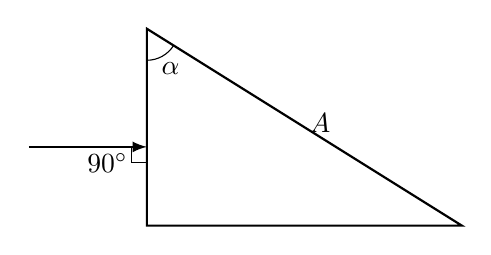
\begin{tikzpicture}[>=latex, scale=1]
    % Prizma (uchburchak)
    \draw[thick] (0,0) -- (0,2.5) -- (4,0) -- cycle;
    
    % To'g'ri burchak belgisi
    \draw (0, 0.8) -- (-0.2, 0.8) -- (-0.2, 1);
    
    \node at (-0.5, 0.8) {$90^\circ$};
    
    % Alfa burchagi
    \draw (0, 2.1) arc (-90:-32:0.4);
    \node at (0.3, 2) {$\alpha$};
    
    % Tomon belgilanishi A
    \node at (2.2, 1.3) {$A$};
    
    % Kelayotgan nur
    \draw[thick, ->] (-1.5, 1) -- (0, 1);
\end{tikzpicture}

\begin{enumerate}[label=\Alph*)]
\item $30^\circ$
\item $15^\circ$
\item $45^\circ$
\item $60^\circ$
\item $75^\circ$
\end{enumerate}

\item Quyidagi shartlardan qaysi biri bajarilganda, yorug‘lik nurining yo‘li rasmdagidek ko‘rinishda bo‘lishi mumkin?

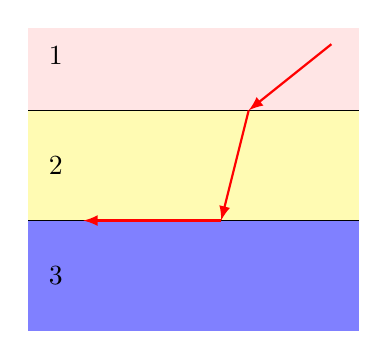
\begin{tikzpicture}[>=latex,scale=0.7]
    % Muhitlarni bo'yash va chizish
    \fill[red!10] (0,4) rectangle (6,5.5); \node at (0.5, 5) {1};
    \fill[yellow!30] (0,2) rectangle (6,4);   \node at (0.5, 3) {2};
    \fill[blue!50] (0,0) rectangle (6,2);   \node at (0.5, 1) {3};
    
    \draw (0,4) -- (6,4);
    \draw (0,2) -- (6,2);
    
    % Nurlar yo'li
    \draw[thick, <-,red] (4, 4) -- (5.5, 5.2); % 1-muhitdan kirish
    \draw[thick, ->,red] (4, 4) -- (3.5, 2);   % 2-muhitda sinish
     % 2-muhitda qaytish
    \draw[thick, ->,red] (3.5, 2) -- (1, 2);   % Chegara bo'ylab yoki 3-muhitga
\end{tikzpicture}

\begin{enumerate}[label=\Alph*)]
\item $n_1>n_2>n_3$
\item $n_2>n_1>n_3$
\item $n_2>n_1=n_3$
\item $n_3>n_2>n_1$
\item $n_2>n_3>n_1$
\end{enumerate}

\item Nurtola (svetovod) larning ish prinsipi nimaga asoslangan?
\begin{enumerate}[label=\Alph*)]
\item yorug‘lik difraksiyasiga.
\item yorug‘lik dispersiyasiga.
\item yorug‘likning sinishiga.
\item yorug‘lik interferensiyasiga.
\item to‘la ichki qaytish hodisasiga.
\end{enumerate}

\item Nuqtaviy yorug‘lik manbai sindirish ko‘rsatkichi $2,24$ bo‘lgan suyuqlik sirtidan $1$ m chuqurlikda joylashgan. Nurlar suyuqlik sirtidan qanday diametrli doira orqali chiqadi (m)?
\begin{enumerate}[label=\Alph*)]
\item $0$
\item $\infty$
\item $0,5$
\item $0,25$
\item $1$
\end{enumerate}

\item Yorug‘lik nuri kvadrat kesimli shisha plastinaga $\alpha$ burchak ostida tushmoqda. Agar plastinaning vertikal joylashgan tomonida to‘la ichki qaytish sodir bo‘lsa, shishaning sindirish ko‘rsatkichi kamida qanday?

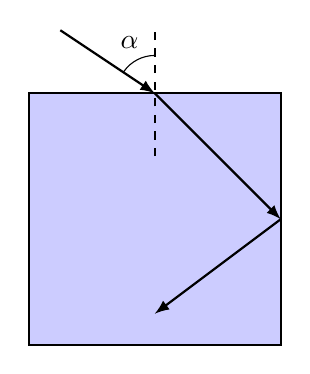
\begin{tikzpicture}[>=latex, scale=0.8]
    % Shaffof blok
    \fill[blue!20] (0,0) rectangle (4,4);
    \draw[thick] (0,0) rectangle (4,4);
    
    % Normal (punktir)
    \draw[dashed, thick] (2, 3) -- (2, 5);
    
    % Nurlar
    \draw[thick, ->] (0.5, 5) -- (2, 4);      % Tushayotgan nur
    \draw[thick, ->] (2, 4) -- (4, 2);        % Ichkarida sinish
    \draw[thick, ->] (4, 2) -- (2, 0.5);      % Yon devordan qaytish
    
    % Alfa burchagi
    \draw (2, 4.6) arc (90:145:0.6);
    \node at (1.6, 4.8) {$\alpha$};
\end{tikzpicture}

\begin{enumerate}[label=\Alph*)]
\item $1+\sin^2\alpha$
\item $\sqrt{1+\sin\alpha}$
\item $\sqrt{1-\sin^2\alpha}$
\item $\sqrt{1+\sin^2\alpha}$
\item $\sqrt{1+\dfrac{1}{\sin^2\alpha}}$
\end{enumerate}

\begin{center}
\begin{tabular}{|c|c|c|c|c|c|c|c|c|c|}
\hline
1c & 2a & 3a & 4e & 5a & 6e & 7b & 8c & 9e & 10a\\
\hline
11d & 12a & 13b & 14d & 15c & 16b & 17b & 18a & 19e & 20c\\
\hline
21a & 22a & 23b & 24e & 25e & 26d & & & & \\
\hline
\end{tabular}
\end{center}
\end{enumerate}



